\documentclass{article}

\usepackage{graphicx}
\graphicspath{ {./images/} }

\usepackage{geometry}
 \geometry{
 a4paper,
 total={170mm,257mm},
 left=20mm,
 top=20mm,
 }

\usepackage{titlesec}

\setcounter{secnumdepth}{4}

\titleformat{\paragraph}
{\normalfont\normalsize\bfseries}{\theparagraph}{1em}{}
\titlespacing*{\paragraph}
{0pt}{3.25ex plus 1ex minus .2ex}{1.5ex plus .2ex}

\usepackage{enumerate}

\usepackage{hyperref}
\hypersetup{
    colorlinks=true,
    linktoc=all,
    citecolor=black,
    filecolor=black,
    linkcolor=black,
    urlcolor=black
}

\usepackage{titleps}

\newpagestyle{main}{
  \sethead
    {\toptitlemarks 1064870 }
    {\thepage}
    {\bottitlemarks Θεόδωρος Συμεωνίδης}
  \setheadrule{.4pt}
}

\pagestyle{main}

\usepackage{fontspec}
\setmainfont{Linux Biolinum}

\title{Εργασία στον Επιστημονικό Υπολογιμό}
\author{Θεόδωρος Συμεωνίδης  \\
	Τμ. Μηχανικών Ηλ. Υπολογιστών και Πληροφορικής}


\begin{document}

\maketitle

\newpage

\tableofcontents

\newpage

% Άσκηση 1
\section{Εισαγωγικά}
\begin{tabular}{ |p{4.5cm}||p{5cm}|}
    \hline
    Χαρακτηριστικό&\\
    \hline
    Έναρξη/Λήξη εργασίας&60\\
    \hline
    model & \\
    \hline
    O/S & Linux version 5.4.11-arch1-1\\
    \hline
    processor name & AMD FX-8350 Eight-Core Processor\\
    \hline
    processor speed& 4.0GHZ (base)\\
    \hline
    total \# cores & 8\\
    \hline
    total \# threads& 8\\
    \hline
    FMA instruction & yes\\
    \hline
    L1 cache& 64 KiB 256 KiB\\
    \hline
    L2 cache& 8 MiB \\
    \hline
    L3 cache& 8 MiB\\
    \hline
    Gflops/s&\\
    \hline
    Memory & 8.117504 kB\\
    \hline
    Memory Bandwidth & 60216.0 MB/s\\
    \hline
    MATLAB version & 9.7.0.1261785 (R2019b) Update 3\\
    \hline
    \end{tabular}

\begin{figure}[h]
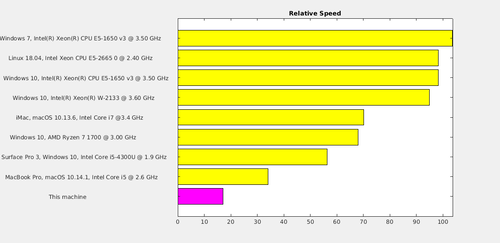
\includegraphics[scale=0.7]{image1}
\end{figure}

\begin{figure}[h]
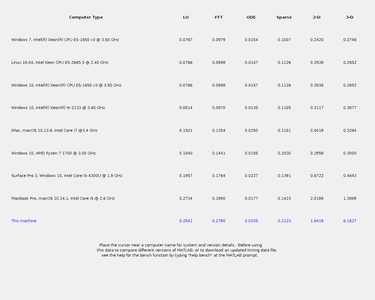
\includegraphics[scale=0.9]{image2}
\end{figure}

\subsection{Κατασκευή Εργαλείων}
\subsection{Μητρώο μάσκα}
\href{run:./mask_band.m}{mask\_band.m}
\subsection{Έλεγχος Διαγώνιας Κυριαρχίας}
\href{run:./dd_check.m}{dd\_check.m}
\subsection{Από MATLAB σε LATEX}
\href{run:./matrix2latex.m}{matrix2latex.m}

% Άσκηση 2
\section{Τανυστές}
\begin{enumerate}[i.]
    \item συντομη περιγραφη της προτασης σας
    \item \href{run:/b2t.m}{b2t.m}
    \item οι τιμες των 4
    \item συντομη περιγραφη της προτασης σας
\end{enumerate}

% Άσκηση 3
\section{Πράξεις με μητρώα ειδικής μορφής, πολυώνυμα μητρώων
και χρήση διεπαφής mex}
\subsection{Μητρώα και δεξιά μέλη}
\begin{tabular}{ |p{4.5cm}||p{1cm}|p{1cm}|p{2cm}|p{1cm}|p{2cm}|p{2cm}|p{1cm}|}
    \hline
    matrix & N & ΔΚ & συμμετρικό & ζώνης & αντιστρέψιμο & δ.κ κ1(Α)\\
    \hline
    $toeplitz([2, -1, zeros(1,8)])$ & 10 & ναι & ναι & (1,1) & ναι & 60\\
    \hline
    $C_{(1000)}$&&&&&&\\
    \hline
    $P_{(100,10)}$&&&&&&\\
    \hline
    $P_{(10,100)}$&&&&&&\\
    \hline
    $P_{(100,100)}$&&&&&&\\
    \hline
    $bcsstm07$ &&&&&&\\
    \hline
    $email$&&&&&&\\
    \hline
   \end{tabular}
\subsection{Επίλυση με απλά πολυώνυμα μητρώου}
\subsubsection{Διαδικασίες επίλυσης}
\begin{enumerate}[i.]
    \item 
    \begin{enumerate}[a.]
        \item \href{run:./chol_btr.m}{chol\_btr.m}
        \item \href{run:./chol_btr_mex.m}{chol\_btr\_mex.m}
        \item κωδικας τυπου script
    \end{enumerate}
    \item 
    \begin{tabular}{ |p{4.5cm}||p{1cm}|p{1cm}|p{2cm}|p{1cm}|p{2cm}|}
        \hline
        RUNTIMES (sec) & $C_{(1000)}$ & $P_{(10,100)}$ & $P_{(100,10)}$ & $P_{100,100}$ & $bcsstm07$\\
        \hline
        explicit &&&&&\\
        \hline
        serial+backslash&&&&&\\
        \hline
        serial+Cholesky&&&&&\\
        \hline
        serial+PCG&&&&&\\
        \hline
        serial+PCG+prec(blockJ)&&&&&\\
        \hline
        \end{tabular}  
        
        
    \begin{tabular}{ |p{4.5cm}||p{1.5cm}|p{1.5cm}|p{1.5cm}|p{1.5cm}|p{2cm}|}
        \hline
        ERRORS (2) & $C_{(1000)}$ & $P_{(10,100)}$ & $P_{(100,10)}$ & $P_{100,100}$ & $bcsstm07$\\
        \hline
        explicit &&&&&\\
        \hline
        serial+backslash&&&&&\\
        \hline
        serial+Cholesky&&&&&\\
        \hline
        serial+PCG&&&&&\\
        \hline
        serial+PCG+prec(blockJ)&&&&&\\
        \hline
        \end{tabular}
\end{enumerate}

% Άσκηση 4
\section{Εφαρμογές σε δίκτυα}
\href{run:./mult_kaltz.m}{mult\_kaltz.m}
\begin{enumerate}[a.]
    \item 
    \begin{tabular}{ |p{4.5cm} p{1cm}||p{1.5cm}|p{2cm}|p{1.5cm}|p{3.5cm}|}
        \hline
        $I-alpha(1)*email$ & $a$ & runtime (sec) & επαναλήψεις & νόρμα & top-5 (hi to lo)\\
        \hline
        format & x.xx & xx.xxxx & xxx & x.xxxxe+xx & π.χ. (1133, 1029, 2, 1, 15)\\
        \hline
        \hline
        explicit & 0.01&&&&\\
        \hline
        & $a_{max}$ &&&&\\
        \hline
        \hline
        $serial+PCG$ & 0.01 &&&&\\
        \hline
        & $a_{max}$ &&&&\\
        \hline
        \hline
        $serial+PCG+prec(ichol)$ & 0.01 &&&&\\
        \hline
        & $a_{max}$ &&&&\\
        \hline
       \end{tabular}

    \item Γρ.Παραστάσεις
    \item Βλέπε πίνακα 1.
\end{enumerate}

\end{document}